\documentclass[aspectratio=169]{beamer}
\input{../utils/beamerpreamble.tex}

\subtitle[Benchmarking Experiment Paper: Part I]{Paper Study -- "Benchmarking in Optimization: Best Practice and Open Issues"\\Part I}
\date{}

\begin{document}

\begin{frame}
  \maketitle

  \vfill

  \hfill \tiny{Version 2024.1 (Updated \today)}
\end{frame}

%%%%%%%%%%%%%%%%%%%%%%%%%%%%%%%%%%%%%%%%%%%%%%%%%%%%%
\section{Outline}

\begin{frame}[t]{Motivation}

  \begin{itemize}
    \item Recent paper describing the best practices in CS experiments involving benchmark analysis;
    \medskip
    
    \item Covers several of the topics of this course: A good review of the topics;
    \medskip

    \item Important for you too: Optimization-like problems occurs in many CS disciplines;
  \end{itemize}

  \vfill

  \begin{block}{}
    Download the paper: https://arxiv.org/abs/2007.03488
  \end{block}
\end{frame}

\begin{frame}{Overview of the Lecture}
  \begin{block}{Today}
    \begin{itemize}
      \item Defining the Goals of a Benchmarking Experiment;
      \item Choosing problems and algorithms;
      \item How to measure the result of the experiment;
    \end{itemize}
  \end{block}
  \begin{exampleblock}{Next Week}
    \begin{itemize}
      \item Types of Analysis;
      \item Experimental Design;
      \item Presentation of the Results;
    \end{itemize}
  \end{exampleblock}
\end{frame}

\begin{frame}[t]{What is an optimization algorithm?}
  Consider a function $\mathbb{R}^N \to \mathbb{R}$. An optimization algorithm finds the input $X \in \mathbb{R}^N$ that minimizes the output.\medskip

  \begin{itemize}
    \item {\bf Applications}: Design of products; Parametrization of Models; System Control; Machine Learning;\medskip

    \item {\bf Classes of Algorithms}: Numerical; Heuristic; Meta-heuristic (search-based); Exhaustive search;\medskip 

    \item {\bf Classes of Problems}: Constrained; Multiple Solutions; Non-continuous; Mixed-Integer; Multiple Objectives;
  \end{itemize}
\end{frame}

\begin{frame}[t]{Benchmark Experiments}
  There is an interest to develop more efficient optimization algorithms. To examine and evaluate new algorithms, optimization researchers often use Benchmark Experiments. \bigskip 

  {\bf Benchmarks} are arbitrary mathematical functions, sometimes based on real world application problems, that are used to test the efficiency of new optimization algorithms.
  \vfill

  \begin{block}{The No Free Lunch Theorem (NFLT) -- Wolpert and Macready, 1997}
    \emph{Optimization algorithms cannot be equally good in all problem classes:}
    \begin{itemize}
      \item Limit analysis of algorithm suitability to the problem {\bf instances} being tested;
      \item Research new problem classes, and match algorithms to specific classes; 
      \item Be careful about generalizing experiment results to other problem instances;
      \item Be {\bf VERY} careful about generalizing results to other problem {\bf classes};
    \end{itemize}
  \end{block}
\end{frame}


%%%%%%%%%%%%%%%%%%%%%%%%%%%%%%%%%%%%%%%%%%%%%%%%%%%%%
\section{Goals of a Benchmarking Experiment (Section 2)}

\begin{frame}[t]{What is a Optimization Benchmarking Study?}
  A "benchmarking study" selects a set of optimization algorithms, a set of benchmark problems, and studies the results of applying the algorithms to the selected problems.
  \bigskip 

  \begin{itemize}
    \item Scientific Motivations: Better understanding of algorithms and problems; 
    \item Engineering Motivations: Find solutions for very specific solutions;
    \item Advertising Motivations: Encourage the use of specific algorithms, problems or technologies;
  \end{itemize}
  \bigskip

  Careful consideration of the study goals plays a {\bf HUGE} role in the selection of algorithms, problems, performance measure, experiment design, analysis, conclusions, etc.
\end{frame}

\begin{frame}{Common Goals of Benchmarking Studies}
  \begin{center}
  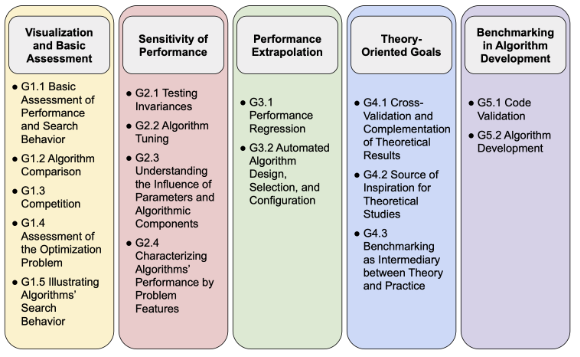
\includegraphics[width=0.7\textwidth]{img/common_goals.png}
  \ppagenote{Table of Benchmarking Studies goal from the "best practices" paper}
  \end{center}
\end{frame}

\begin{frame}{1- Visualization and Basic Assessment}
  \begin{itemize}
    \item {\bf 1.1 - Basic Assessment of Performance and Behavior}: How does one specific Algorithm Configuration performs at one specific Problem Instance? Considerations for Stochasticity and robustness. Considerations for evaluation measures;
    \item {\bf 1.2 - Algorithm Comparison}: Most common in literature. Extension of the above for multiple Algorithms / Algorithm Configurations. Specify the most suitable algorithm configuration for a problem class or instance;
    \item {\bf 1.3 - Competition}: Compare several algorithms on specific set of problem instances, and specific performance measures; Can promote development of new ideas, but can also overfit/exaggerate the importance of certain problems/measures;
    \item {\bf 1.4 - Assessment of Problem}: Improve the understanding of a problem: How close is the benchmark function to reality? What is the class of the problem? What is the fitness landscape? How difficult is the problem?
    \item {\bf 1.5 - Illustrating the Search Behavior}: What is the robustness of the algorithm? How fast does it converge? What are the characteristics of its behavior?
  \end{itemize}
\end{frame}

\begin{frame}{2- Sensitivity of Performance}
  \begin{itemize}
    \item {\bf 2.1 - Testing Invariances}: Testing if the performance of the algorithm is invariant to certain characteristics of the problem (eg: translation invariance)
    \item {\bf 2.2 - Algorithm Tuning}: Fiding the most suitable configuration (parameters and hyper parameters) of an algorithm to a specific instance or class of problem;
    \item {\bf 2.3 - Understanding the influence of parameters}: How does the performance of the algorithm changes with the change of parameters. What parameters have higher or lower influence, depending on the problem instance? What is the specific effect of a parameter on the algorithm or problem instance? Compare with 2.2.
    \item {\bf 2.4 - Characterizing the algorithm by problem feature}: Related to 2.3, how does the characteristics of a problem class/instance affect the algorithm's performance? What characteristics have higher or lower effect on the algorithm?
  \end{itemize}
  
\end{frame}

\begin{frame}{3- Benchmark as Training: Performance Extrapolation}
  \begin{itemize}
    \item {\bf 3.1 - Performance Regression}: Extrapolating the performance of the algorithm from problem classes and instances that were tested, to problems classes and instances that were not tested. How much {\bf can we expect} the performance of the algorithm to change or degrade? How do we select problems to evaluate this degradation? \emph{Related to ideas of train/testing, transfer learning, and zero shot in Machine Learning}; \bigskip
    
    \item {\bf 3.2 - Automated Algorithm Design, Selection and Configuration}: If we know the influence of parameter configuration and problem characteristics to an algorithm, it should be possible to automatically select appropriate parameters from the characteristics of an unseen problem instance. The goal of this kind study is to develop training data and guidelines to such a task, given an automated configuration framework.
  \end{itemize}
\end{frame}

\begin{frame}{4- Theory Oriented Goals}
  \begin{itemize}
    \item {\bf 4.1 - Complementation of Theoretical Results}: Replication, Confirmation, and Extension of theoretical results for larger problems;
    \item {\bf 4.2 - Inspiration for Theoretical Studies}: Studies in a large quantity of problems or algorithms to observe patterns, and then try to explain those patterns through theoretical construction. The theory can explain, extend, or bound the experimental observations.
    \item {\bf 4.3 - Bridge between theory and practice}: Transform knowledge from theory into actual algorithms that are applicable to specific problems with specific issues;
  \end{itemize}
\end{frame}

\begin{frame}{5 - Benchmark in Algorihtm Development}
  \begin{itemize}
    \item {\bf 5.1 - Source Code Validation}: Verify that a program (instance of algorithm) performs as expected (theory or literature results). If the program does not behave as expected from past knowledge, this indicates the necessity of a code review, and the existence of bugs.\medskip 
    
    \item {\bf 5.2 - Algorithm Development}: Benchmark studies can be used to identify weak spots in the literature, and to find the needs for new algorithms and methods. This includes initial empirical examinations of new ideas, fine-tuning future research directions.
  \end{itemize}
  \bigskip
  
\end{frame}


\begin{frame}{What are all these objectives good for?}
  \begin{itemize}
    \item Think about your scientific objective carefully: Most people automatically go for comparison studies, but for some scientific questions, other kinds of studies might be more appropriate;
    
    \item Think about your experiment design carefully: Depending on the kind of study, the way you design the experiment will change. Having a clear vision of the goal of the study is important. Also you can compare to similar studies (if you know what those studies are)
  \end{itemize}

  \begin{block}{Short Exercise: How does this apply to you?}
    Consider experiments that you have performed so far (in this course, or in your master research). How would you classify the goal of that experiment? Would a different goal have been more useful to you? How do you transform some of these goals into your discipline?
  \end{block}
\end{frame}

% A lot of papers focus on "comparison" and "competition", but we need to know many more things. Example: experiments on iris.

%%%%%%%%%%%%%%%%%%%%%%%%%%%%%%%%%%%%%%%%%%%%%%%%%%%%
\section{Selection of Problems and Algorithms (Section 3 and 4)}

\begin{frame}[t]{Selecting Problems and Algorithms}
  After selecting the objective of the study, we need to choose the algorithms (algorithm configurations) under study, and the problem set (problem classes, problem instances);
\end{frame}

\subsection{Problems}

\begin{frame}[t]{Problem Class vs Problem Instance}
  \begin{itemize}
    \item A {\bf problem / problem class} specifies the general characteristics of the given optimization problem: Is it unimodal/multimodal? Is it continuous/discrete? What function represents the problem? \medskip
    
    \structure{Example:} The "Sphere" function;\medskip
    \item A {\bf problem instance} specifies the implementation of one specific case of the problem class. It can include the values for constants in the problem formula, which can be changed to generate new instances. Or the number of dimensions or scale of the problem. \alert{Different instances of the same problem class can have different difficulty}!\medskip 
    
    \structure{Example:} The 5-dimensional sphere function $f: \mathbb{R}^5 \to \mathbb{R}, x\to\alpha\sum^d_{i=1}x^2_i+\beta$, centered at the origin, with multiplicative parameter $\alpha$ and shift parameter $\beta$.
  \end{itemize}
\end{frame}

\begin{frame}[t]{Problem Set}
  In general, the goal of a benchmark study include understanding the performance of algorithms not on one problem instance, but on a variety of problems instances and classes. Therefore, we need to always consider the {\bf Problem Set} of an study:
  \bigskip

  Problem Set:
  \begin{itemize}
    \item Problem Class A
    \begin{itemize}
      \item Problem A1
      \begin{itemize}
        \item Problem Instance A1-a 
        \item Problem Instance A1-b 
        \item Problem Instance A1-c
      \end{itemize}
      \item Problem A2
      \item Problem A3
    \end{itemize}
    \item Problem Class B
    \item Problem Class C 
  \end{itemize}
  
\end{frame}

\begin{frame}{Desirable Characteristics of a Benchmark Problem Set}
  \begin{itemize}
    \item {\bf Diverse:} Different difficulties, different classes, different characteristics;
    \item {\bf Representative:} Correspond to difficulties and characteristics encountered in real world problems;
    \item {\bf Scalable / Tunable:} By changing parameters, we can increase or decrease the difficulty, or generate variations of the same class of problems, as necessary.
    \item {\bf Known Solutions / Performance:} We know some target values (absolute or relative) that the algorithm should reach if performing well;
  \end{itemize}
\end{frame}

\begin{frame}[t]{Evaluating the Quality of a Problem Set}
  How can we evaluate the characteristics (diversity, representation, scalability) of a problem set? \bigskip 

  Some past research approaches:
  \begin{itemize}
    \item Clustering of characteristics of problem instances;
    \item Clustering of performance of algorithms on the problem set;
    \item Automated creation and analysis of problem instances;
    \item Sensitivity analysis focused on {\bf problem/problem instance} (How easy a problem gets as a parameter changes)
    \item Analysis of past results in the literature (are new algorithms obtaining significative changes in results?)
  \end{itemize}\bigskip 

  The result of this kind of research can provoke the creation of new benchmark sets to cover quality issues in old benchmark sets. 
  
\end{frame}

% Problems instances and problem classses

\subsection{Algorithms}

\begin{frame}[t]{Generalization: Algorithm vs Algorithm Configuration}

  It is important to consider if our studies and experiments give us information about an algorithm, or about a specific instance of an algorithm:\medskip

  \begin{itemize}
    \item {\bf Algorithm}: The CMA-ES algorithm;
    \item {\bf Algorithm Configuration}: The pycma-es implementation, with population size 8, budget 100, restart strategy X, etc... 
  \end{itemize}\bigskip 

  The performance of an algorithm can vary intensely depending on its implementation and configuration.
  
\end{frame}

\begin{frame}[t]{Generalization: Hyperparameter Handling}
  The performance of algorithm configurations depends on the hyperparameter settings and the problem characteristics. Because of this, it is necessary to tune all algorithms involved in a study.\bigskip 

  {\bf "Literature Parameters"}: Even if an algorithm has been tuned in a different study from the literature, there are interaction effects between the algorithm configuration and the problem characteristics. These interaction effects require the re-tuning to guarantee an accurate evaluation of the performance of an algorithm (configuration) on a benchmark set. (Also, use parameter fine-tuning tools such as iRACE and SMAC)\bigskip

  \begin{exampleblock}{Question}
    In what experimental situations the fine tuning of algorithms (i.e., the use of "literature parameters") would be sufficient? What should be considered in those situations?
  \end{exampleblock}
\end{frame}

\begin{frame}[t]{Algorithm characteristics and the "State of the Art"}
  Many studies involve the comparison of several algorithms. The choice of algorithms should be influenced by several factors:
  \begin{itemize}
    \item \structure{Problem features}: Different algorithms are appropriate for different problem classes and feature. A literature review is important for this choice, along with preliminary experiments to evaluate the properties of the algorithm on the problem.\medskip 
    
    \item \structure{State of the Art}: As technology develops, it is important to compare algorithms against the most recent version {\bf and implementation} of classical algorithms. Searching for the state of the art from algorithm competitions is also recommended. Note that the state of the art may depend on the problem's characteristics;
  \end{itemize}
\end{frame}

\begin{frame}{Other factors regarding algorithm selection}
  \begin{itemize}
    \item \structure{Optimization Budget}: Optimization Budget is the amount of computation available for performing an optimization task (usually in terms of fitness evaluations). Different algorithms may perform better with low budgets (surrogate optimization algorithms) vs high budget (Evolution Strategy algorithms). This is an example of how problem characteristics affect the choice of state-of-the-art.

    \item \structure{Initialization}: Optimization performance depends heavily on the initial conditions (starting close to the optimal may improve the results). Therefore all algorithms should have the same starting conditions, and a variety of starting conditions (seeds) should be examined to avoid "coincidental" results.
  \end{itemize}\bigskip

  In general, the choice of competing algorithm should be analyzed carefully, and informed by the goal of the experiment.
\end{frame}


% Difference between "algorithms" and "algorithm instances"

%%%%%%%%%%%%%%%%%%%%%%%%%%%%%%%%%%%%%%%%%%%%%%%%%%%%
\section{Measuring Performance (Section 5)}

\begin{frame}[t]{Measuring Performance}
  Optimization Benchmark Experiments usually ask one of two questions:
  \begin{itemize}
    \item "How fast can the algorithms achieve a given solution quality?"
    \item "What solution quality can the algorithms achieve with a given budget?"
  \end{itemize}

  \begin{columns}
    \column{0.6\textwidth}
    The most common way to visualize the result of an optimization algorithm is a graph with the computation budget on the x-axis, and the performance measure on the y-axis. 
    \column{0.4\textwidth}
    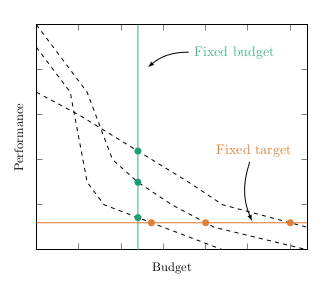
\includegraphics[width=1\textwidth]{img/budget_performance.png}
    \ppagenote{Budget Performance graph from "Best Practices" paper}
  \end{columns}
\end{frame}

\begin{frame}{Measuring Budget}
  The budget of an algorithm can be measured in different ways:
  \begin{itemize}
    \item {\bf Time}: Wall clock time, or CPU time; (Important when the optimization problem can be evaluated very quickly, eg: SAT)
    \item {\bf Functions Evaluations}: How many times the optimization function was called (important when the optimization problem cannot be evaluated quickly, eg: simulations)
  \end{itemize}  
\end{frame}

\begin{frame}[t]{Measuring Solution Quality}
  \begin{itemize}
    \item There are many \structure{problem-specific} measures of solution quality;
    \begin{itemize}
      \item Comparing quality across problems becomes an issue;
    \end{itemize}
    \item Generalized solution quality: Distance (absolute or relative) to optimal solution;
    \begin{itemize}
      \item Method for obtaining relative distance (normalization) can be an issue;
    \end{itemize}
    \item Number of constraints violation;
  \end{itemize}
  
\end{frame}

\begin{frame}[t]{Measuring Algorithm Robustness}
  Reasons for volability (change) in repeated results: 
  \begin{itemize}
    \item Stochastic behavior of algorithm (random search, random factors in algorithm);
    \item Initial condition of the optimization (seed, initial population);
    \item Noisy problem (stochasticity of the problem, change in data sets, physical conditions)
  \end{itemize}\bigskip

  Measuring Robustness of algorithm performance:
  \begin{itemize}
    \item {\bf With Fixed Budget:} Mean or median of the algorithm performance across multiple repetitions;
    \item {\bf With Target performance:} Count of failed/successful runs; Expected Running Time (ERT) measure; Penalized Average Runtime (PAR/PQR) measure;
    \item {\bf Quantiles, Standard Deviations, Confidence Intervals:} Smaller measures of variability in the results indicate higher robustness; 
  \end{itemize}
  
\end{frame}


%%%%%%%%%%%%%%%%%%%%%%%%%%%%%%%%%%%%%%%%%%%%%%%%%%%%
\section{Summary}

\begin{frame}{Summary}
  \begin{itemize}
    \item {\bf Selecting the goal of the experiment}: The goal of an algorithm experiment can be much more than "compare two algorithms".

    \item {\bf Selecting algorithm and problem sets}: Algorithms and Problem Sets will affect each other, and should be chosen carefully. Difference between algorithm and algorithm instance, problem and problem instance;
    
    \item {\bf Performance Measures}: There are many ways to measure the performance of an algorith. Fixed budget vs Fixed target evaluation. Evaluation of Robustness.
  \end{itemize}
  
\end{frame}

\begin{frame}{Exam and Final Report}
  \begin{itemize}
    \item {\bf Exam:} I hope to give an example exam next class (maybe only on manaba). The topics are the contents of all lectures (including these two lectures). Calculations will not be necessary. 
    
    \item {\bf Final Report:} I will post the final report to Manaba ASAP. It will involve performing 
  \end{itemize}
  
\end{frame}


%%%%%%%%%%%%%%%%%%%%%%%%%%%%%%%%%%%%%%%%%%%%%%%%%%%%
\input{../utils/lastslide.tex}
\end{document}